Extreme value theory uses the limited information available in a sample to
    characterize the tails of a distribution.  In the univariate case, asymptotic
    results provide a unique parametric limiting family for the maximum observation
    in a sample.  For data with such a limiting distribution, a common approach
    is to consider observations in excess of a high threshold, and model the
    excesses over that threshold under a generalized Pareto framework.  This
    approach is known as \emph{peaks over threshold} (PoT).  In the multivariate 
    case, the theory for PoT is well established (see, for example, 
    \cite{dehaan2006}), and it indicates the existence of a limiting distribution
    with no parametric representation.  This can pose a challenge for inference,
    but we are not without options.

The multivariate PoT model considered in this paper has been developed 
    in~\cite{trubey:pg}, based on a definition of the limiting distribution proposed
    proposed in~\cite{rootzen2018}.  
    Let $\bm{W} = (W_1,\ldots,W_d)$ be a $d$--dimensional random vector with 
    cumulative distribution $F$.  Assuming there exists a sequence of vectors
    $\bm{a}_n$, $\bm{b}_n$, and a $d$--variate distribution $G$ such that 
    $\lim\limits_{n\to\infty}F^n(\bm{a}_n\bm{w} + \bm{b}_n) = G(\bm{w})$, then
    $G$ is a $d$--variate generalized extreme value distribution.  Then,
    \begin{equation}
        \label{eqn:threshold}
        \lim\limits_{n\to\infty}\text{Pr}
            \left[\bm{a}_n^{-1}(\bm{W} - \bm{b}_n) 
                \leq \bm{w}\mid \bm{W}\not\leq \bm{b}_n\right]
        = \frac{\log G(\bm{w}\wedge \bm{0}) - \log G(\bm{w})}{\log G(\bm{0})}
        = H(\bm{w})
    \end{equation}
    where $H$ is the multivariate Pareto distribution.  \cite{rootzen2018}
    provides a number of stochastic representations of $H$, and in particular,
    Remark~1 justifies the representation given in \cite{ferreira2014} where,
    in the limit, we factorize $\bm{W} = R\bm{V}$ with $R$ and $\bm{V}$ independent.
    % \makenote{I'm not very fond of this transition.  We standardize $\bm{W}$ to 
    % $\bm{Z}$, then factorize $\bm{Z} = R\bm{V}$.  Separability holds true in both
    % cases (i think), but in the former, $\bm{V}$ is still dependent on the marginal 
    % distributional parameters.  Standardization allows those to be ignored.  Or
    % sidelined.  We should mention standardization before factorization.}
    $R = \lVert \bm{W}\rVert_{\infty}$ is distributed as a standard Pareto random
    variable, and $\bm{V} = \bm{W} / \lVert \bm{W}\rVert_{\infty}$ is a random
    vector existing within $\mathbb{S}_{\infty}^{d-1}$, the positive orthant of
    the unit sphere under the $\mathcal{L}_{\infty}$ norm.  $R$ and $\bm{V}$
    respectively comprise the \emph{radial} and \emph{angular} components of $H$.
    As $R$ and $\bm{V}$ are independent,  the distribution of $\bm{V}$ is 
    effectively the dependence structure of $\bm{W}$.

We consider observations $\bm{w}_{i} = (w_{i1}, \ldots , w_{iS})$, where 
    $i =1 ,\ldots m ,n$. For the case of the SLOSH simulations, $i$ indexes 
    storms, and $s$ indexes the grid cell in the simulation output.
    Define as the threshold $b_{qs} = \hat{F}_{s}^{-1}(1 - q)$, where $\hat{F}$ is
    the empirical cumulative distribution function for the $s$th component.
    Marginally, values exceeding the threshold $b_{qs}$ are assumed to follow
    a univariate generalized Pareto distribution, and are used to estimate the
    corresponding marginal scale and shape parameters $a_{s}$ and $\xi_{s}$
    respectively.  Let
    \begin{equation}
        \label{eqn:standardization}
        z_{is} = \left(1 + \xi_{s}\frac{w_{is} 
            - b_{s}}{a_{s}}\right)_{+}^{1 / \xi_{s}}
    \end{equation}
    where $(\cdot)_+$ indicates the positive parts function.  Let 
    $r_i = \lVert \bm{z}_i\rVert_{\infty}$, and $\bm{v}_i = \bm{z}_i / r_i$.  Due to 
    thresholding, $i$ ranges from 1 to $m\leq n$, and $r_i > 1$.  The core 
    assumption of our model is the use of $\bm{v}_i$ to describe the 
    angular component of the tail distribution that corresponds to the
    observations.

\subsection{Projected Gamma\label{sec:pg}}
A suitable distribution for $\bm{V}$ can be approximated by projecting a 
    distribution in $\mathbb{R}_+^d$ onto $\mathbb{S}_{p}^{d-1}$.  
    Recall the $\mathcal{L}_p$ norm 
    $\lVert \bm{x}\rVert_p = \left(\sum_{s = 1}^dx^p\right)^{1/p}$.  Then
    for $\bm{x}\in\mathbb{R}_+^d$, we define the transformation
    \begin{equation}
        \label{eqn:projection}
        T_p(\bm{x}) = \left(\lVert \bm{x}\rVert_p, 
            \frac{x_1}{\lVert \bm{x}\rVert_p},\ldots, 
                \frac{x_{d-1}}{\lVert \bm{x}\rVert_p}\right)
                =: (r,\bm{y})
    \end{equation}
    where $y = (y_1,\ldots,y_{d-1}) \in \mathbb{S}_{p}^{d-1}$, $r > 0$, and 
    $y_d = (1 - \sum_{s = 1}^{d-1}y_{s}^p)^{\frac{1}{p}}$.
    By transforming $\bm{x}$ to $(r,\bm{y})$ and integrating out $r$, we
    obtain a distribution for $\bm{y}$ on $\mathbb{S}_{p}^{d-1}$.
    The Jacobian of the transformation in Equation~\eqref{eqn:projection} is
    $r^{d-1}[Y_d + \sum_{s = 1}^{d-1}y_{s}^py_d^{1-p}]$.
    This Jacobian is well suited to a product of gammas density, where 
    $f(\bm{x}\mid\bm{\alpha},\bm{\beta}) = 
        \prod_{s = 1}^d\mathcal{G}(x_{s}\mid\alpha_{s},\beta_{s})$.
    Transforming $\bm{x}$ as described, $r$ can be integrated out in closed
    form, yielding the \emph{projected gamma} density for arbitrary $p > 0$,
    \[
        f(\bm{y}\mid\bm{\alpha},\bm{\beta}) = \prod_{s = 1}^d\left[
            \frac{\beta_{s}^{\alpha_{s}}}{\Gamma(\alpha_{s})}
            y_{s}^{\alpha_{s} - 1}\right]
            \left[y_d + \sum_{s = 1}^{d-1}y_{s}^py_d^{1-p}\right]
            \frac{\Gamma(\sum_{s = 1}^d \alpha_{s})}{\left(
                \sum_{s = 1}^d\beta_{s}y_{s}
                \right)^{\sum_{s = 1}^d \alpha_{s}}
            }.
    \]
    Unfortunately, at $p=\infty$, the transformation is not differentiable, so a 
    direct projection onto $\mathbb{S}_{\infty}^{d-1}$ is not possible. Yet,
    as $p\to\infty$, $\mathbb{S}_{p}^{d-1}$  will approach $\mathbb{S}_{\infty}^{d-1}$.
    Unfortunately, as $p\to\infty$, the stability of the Jacobian of the transformation 
    becomes increasingly dependent on the value, or choice, of $y_d$.  If 
    $y_d\to 0$, then the Jacobian diverges, and the distribution becomes numerically 
    unstable. We select $p = 10$ to balance these concerns.

To more flexibly capture the structure of the data, we use the projected gamma density 
    as a kernel density of a Bayesian non-parametric mixture model, based on 
    the Pitman-Yor process introduced in~\cite{perman1992}.  A Pitman-Yor process
    is a fully atomic measure specified by two parameters and a centering
    distribution.  Under a stick-breaking representation as described 
    in~\cite{ishwaran2001}, 
    \begin{equation}
        \label{eqn:stickbreak}
        \text{Pr}(\bm{\alpha}\mid\ldots) 
            = \sum_{j = 1}^Jp_j\delta_{\bm{\alpha}_j};\;\;\;
            \sum_{j=1}^Jp_j = 1;\;\;\;
            p_j \coloneqq\chi_j\prod_{k = 1}^{j-1}(1 - \chi_k)
    \end{equation}
    where $\delta_{\bm{\alpha}_j}$ indicates a point mass at $\bm{\alpha}_j$ and
    $\bm{\alpha}_j$ are sampled independently from the centering distribution $G_0$.
    Under the Pitman-Yor process, $\chi_j \sim \text{Beta}(1 - d, \eta + jd)$
    where $d \in [0, 1)$ denotes the \emph{discount} parameter and $\eta > -d$
    denotes the \emph{concentration} parameter. Notice that $J$ denotes a
    truncation for the number of mixture components and, thus, $j\in \lbrace 1,\ldots,J\rbrace$ 
    denotes indexing over \emph{clusters}.

Let $y_{is}$ be the storm surge at location $s$ during storm $i$, after thresholding and projection 
    onto $\mathbb{S}_p^{d-1}$.  Then, the model can be specified as
    \begin{equation}
        \label{eqn:pypg}
        \begin{aligned}
            \bm{y}_i \mid \bm{\alpha}_i &\sim
                \mathcal{PG}_p\left(\bm{Y}\mid\bm{\alpha}_i,\bm{1}\right)\\
            \bm{\alpha}_i &\sim G\\
            G &\sim \mathcal{PY}\left(\eta, \zeta, G_0\right)        
        \end{aligned}
        ~\hspace{1cm}
        \begin{aligned}
            G_0 &= {\textstyle\prod}_{s = 1}^{S}\mathcal{G}(\alpha_{s}\mid \xi_{s},\tau_{s})\\
            \xi_{s} &\sim \mathcal{G}(\xi\mid a, b)\\
            \tau_{s} &\sim \mathcal{G}(\tau\mid c, d)
        \end{aligned} 
    \end{equation}
    where $\eta$ and $\zeta$ are respectively the concentration and discount parameters
    of the Pitman--Yor process.  Fitting this model can be accomplished via Markov-chain 
    Monte Carlo methods. We can introduce a latent cluster assignment variable $\delta_i$ 
    such that 
    $\text{P}\left(\delta_i = j\mid\bm{y},\bm{\alpha}\right) = 
        \text{P}\left(\bm{\alpha}_i = \bm{\alpha}_j\mid \bm{y},\bm{\alpha}\right)$ as described in 
        Equation~\eqref{eqn:stickbreak}.
    Then the full conditional distribution of $\delta_i$ conditional on $\bm{\chi}$ is
    \begin{equation}
        \label{eqn:pdelta}
        \text{P}\left(\delta_i = j\mid \bm{y},\bm{\alpha},\bm{\chi}\right) = 
            \frac{p_j\mathcal{PG}(\bm{y}_i\mid\bm{\alpha}_j)}{
                \sum_{k = 1}^J p_k\mathcal{PG}(\bm{y}_i\mid\bm{\alpha}_j)}
    \end{equation}
    and the full conditional of $\chi_j$ conditional on $\bm{\delta}$ is
    \begin{equation}
        \label{eqn:pchi}
            \chi_j\mid\bm{\delta} \sim \mathcal{B}\left(\zeta_{\chi_j 1} = 1 + n_j - d,\; 
                            \zeta_{\chi_j 2} = {\textstyle \sum}_{k>j} n_k + \eta + jd\right)
    \end{equation}
    where $p_j = \chi_j\prod_{k=1}^{j-1}(1 - \chi_k)$,  as described in in 
    Equation~\eqref{eqn:stickbreak}, and $n_j = \sum_{i = 1}^n\bm{1}_{\delta_i = j}$.
    % \bruno{\bf I got lost here. What is $\bm{\nu}$?}
    We can further introduce a latent $r_i\mid \bm{y}, \delta_i,\bm{\alpha} \sim 
        \mathcal{G}\left(r\mid \sum_s \alpha{\delta_is},\sum_s y_{is}\right)$ such that the
    likelihood of $\bm{\alpha}_j$ becomes separable by dimension.  Posterior updates 
    for $\bm{\alpha}$, and $\bm{\xi}$ can be accomplished via Metropolis-within-Gibbs steps,
    and the full conditional of $\tau_s$ has a known form as a Gamma distribution.

Such a fitting scheme can work well for a moderately sized inference problem.  In \cite{trubey:pg},
    they report requiring approximately \num{20} minutes to run the sampler for \num{40000} iterations, 
    on a problem with \num{532} observations $\times$ \num{47} sites.  If we want to conduct
    MCMC inference for more sites, and more observations, the sampler may need more iterations to
    reach convergence, each iteration will require more CPU time, and the sampler will have an 
    increasing memory footprint. Thus, we consider, as an alternative, a variational inference approach.

\subsection{Variational Inference - A Brief Overview\label{sec:varbayes}}
Variational inference, or variational Bayesian statistics, is an alternative method of 
    model-fitting that proposes, if the target distribution is analytically intractable,
    to fit a tractable candidate distribution as \emph{close} to the target distribution
    as possible \citep{blei2017}. That is, for data $\bm{x}$ and some 
    distributional parameter set $\bm{\theta}$, where $f(\bm{\theta}\mid \bm{x})$ is not 
    available in closed form, we select $q(\bm{\theta})$ from a family of tractable distributions
    $\bm{Q}$.  Variational inference selects the \emph{optimal} variational distribution $q^*$
    by minimizing the KL divergence.  Thus,
    \begin{equation}
        \label{eqn:optimalq}
        q^*(\bm{\theta}) = \argmin_{q\in\mathcal{Q}}\left\lbrace
        \text{KL}\left(q(\bm{\theta})||f(\bm{\theta}\mid\bm{x})\right) 
        \coloneqq
        \text{E}_{q}\left[\log\left(
        \frac{q(\bm{\theta})}{f(\bm{\theta}\mid\bm{x})}
        \right)\right]
        \right\rbrace.
    \end{equation}
    There are myriad flavors of variational approaches, differentiating by
    the type and degree of structure, or dependence, they allow between the parameters in
    the variational distribution, or in the specific method they use to fit the variational
    distribution.  Of particular note here is \emph{mean field} variational Bayes, which 
    holds each parameter's variational distribution as independent of that from all other 
    parameters in the model.  That is,
    \[
        q_{\bm{\theta}} = \prod_{\ell \in L}q_{\theta_{\ell}}(\theta_{\ell}\mid\psi_{\ell})
    \]
    If we hold each $q_{\theta_{\ell}}$ to be an appropriate transformation of a normal
    distribution, then each $q_{\theta_{\ell}}$ can be specified by a mean and variance 
    parameter. 
    % Some \needcite more complicated flavors of variational Bayes will relax 
    % this independence restriction.

Through analytic manipulation we can separate the KL divergence into two quantities: the 
    evidence $\log f(x)$, and the negative of the evidence lower bound, or \emph{ELBO},
    \begin{equation}
        \label{eqn:elbo}
        \mathcal{L}(\bm{\theta}) = 
            \text{E}_q\left[\log f(\bm{x},\bm{\theta}) - \log q(\bm{\theta})\right] 
                = \text{E}_q[\log f(\bm{x},\bm{\theta})] - H,
    \end{equation}
    where $H$ denotes the entropy of $q$.  As the evidence is constant with respect 
    to $q$, minimizing the KL divergence is equivalent to maximizing the ELBO, so 
    restating Equation~\eqref{eqn:optimalq}, we get
    \begin{equation}
        \label{eqn:optimalq2}
        q^*(\bm{\theta}) = \argmax_{q\in\mathcal{Q}} \mathcal{L}(\bm{\theta}).
    \end{equation}
    For a given family $Q$, finding the optimal $q^*$ means finding the optimal parameter set 
    $\bm{\psi}^*$ such that $q^*(\bm{\theta}) = q(\bm{\theta}\mid\bm{\psi}^*)$.
    For continuous parameters, optimization of the ELBO with respect to $\bm{\psi}$ can be 
    accomplished by analytically computing the gradient,
    \begin{equation}
        \label{eqn:gradient}
        \Delta_{\bm{\psi}} = \frac{\partial}{\partial \psi_{\ell}}
            \left\lbrace\text{E}_{q}\left[\log f(\bm{y}\mid\bm{\theta})\right] 
                - H(\bm{\psi})\right\rbrace
            \;\;\text{ for }\ell = 1,\ldots,d, 
    \end{equation}
    then iteratively moving towards the optimal point, where $\Delta_{\bm{\psi}} = \bm{0}$.  
    As the above expectation is not available in closed form for our model, we make implicit 
    use of the reparametrization gradient \citep{kingma2022}, that takes samples of $\bm{\theta}$ 
    as a function of $\bm{\psi}$ and an independent R.V. $\epsilon$.  This allows us to move
    the differentiation inside the expectation, and take the expectation numerically.  To do 
    the optimization, we use the well-regarded \emph{Adam} optimizer \citep{kingma2017}, a combination of 
    \emph{ADAGRAD} \citep{duchi2011} and \emph{RMSProp} \citep{tieleman2012}.  Adam is stated to be 
    well-suited to noisy and high-dimensional problems, and this problem likely fits the criteria.
    That said, a path-based optimization approach will be dependent upon the starting position,
    and if multiple local optima exist, there is no guarantee of reaching the
    global optimum value.  In our analysis, results are highly dependent upon starting position, 
    both in terms of model fidelity, and the resulting number of extant mixture components.  
    One solution would be to consider a better starting position for the optimizer. 

% To expand, using KL divergence as an analogue to distance, variational inference attempting 
%     to find the \emph{closest} tractable surrogate posterior $q$ within the family 
%     $\mathcal{Q}$ to the true posterior.  
%     As has been explained however, we do not necessarily have 
%     $f(\bm{\theta}\mid\bm{y})$ directly.  Let 
%     $f(\bm{y},\bm{\theta}) = f(\bm{y}\mid\bm{\theta})f(\bm{\theta})$.
%     Then we reformulate the KL divergence into
%     \[
%         \begin{aligned}
%         \text{KL}\infdiv{q(\bm{\theta}\mid\bm{\psi})}{f(\bm{\theta}\mid\bm{x})}
%             &=\text{E}_{\bm{\psi}}\left[\log\left(
%                 \frac{q(\bm{\theta}\mid\bm{\psi})}{f(\bm{\theta}\mid\bm{x})}
%                 \right)\right] = \text{E}_{\bm{\psi}}\left[
%                 \log\left(\frac{q(\bm{\theta}\mid\bm{\psi})f(\bm{x})}{f(\bm{y},\bm{\theta})}
%                 \right)\right]\\
%             &= \text{E}_{\bm{\psi}}\left[
%                 \log q(\bm{\theta}\mid\bm{\psi}) - \log f(\bm{x},\bm{\theta}) 
%                 + \log f(\bm{x})
%                 \right]\\
%             &= \text{E}_{q}\left[
%                 \log q(\bm{\theta}) - \log f(\bm{x},\bm{\theta})\right] + 
%                    \log f(\bm{x}).
%         \end{aligned}
%     \]
%     Note that the second term, the \emph{evidence}, is constant with respect to 
%     $\bm{\theta}$.  With a bit of rearrangement,
%     \[
%         \begin{aligned}
%         \log f(\bm{x}) 
%             &= \text{KL}\infdiv{q(\bm{\theta})}{f(\bm{\theta}\mid\bm{x})}
%                 - \text{E}_q\left[
%                 \log q(\bm{\theta}) - \log f(\bm{x},\bm{\theta})
%                 \right]\\
%             &= \text{KL}\infdiv{q(\bm{\theta})}{f(\bm{\theta}\mid\bm{x})}
%                 + \mathcal{L}(\bm{\theta})
%         \end{aligned}
%     \]
%     Thus maximizing $\mathcal{L}(\bm{\theta})$ is equivalent to minimizing the 
%     KL divergence. In this form, as KL divergence is a positive quantity, it is
%     readily apparent that $\mathcal{L}(\bm{\theta})$ establishes a lower bound
%     on the evidence, and maximizing said lower bound is equivalent to minimizing
%     the KL divergence.  Thus the variational literature has christened it the
%     \emph{evidence lower bound}, often abbreviated to \emph{ELBO}.  As such,
%     we can rewrite Equation~\eqref{eqn:optimalq} to
%     \[
%         q^*(\bm{\theta}) = \argmax_{q\in\mathcal{Q}} \mathcal{L}(\bm{\theta})
%     \]
%     Note that we specify $q$ so as to depend on a set of variational parameters 
%     $\bm{\psi}$, such that choosing the optimal $\bm{q}$ means in effect choosing
%     the optimal $\bm{\psi}$.  

% Optimization of the ELBO with respect to $\bm{\psi}$ can be accomplished by
%     analytically computing the gradient,
%     \begin{equation}
%         \label{eqn:gradient}
%         \Delta_{\bm{\psi}} = \frac{\partial}{\partial \psi_{\ell}}
%             \left\lbrace\text{E}_{q}\left[\log f(\bm{y}\mid\bm{\theta})\right] 
%                 - H(\bm{\psi})\right\rbrace
%             \;\;\text{ for }\ell = 1,\ldots,d,
%     \end{equation}
%     where $H(\bm{\psi})$ is the entropy of $q$, and, subject to some conditions \makenote{rephrase},
%     locating the optimal point where $\Delta_{\bm{psi}} = \bm{0}$.  However, when 
%     $\Delta \text{E}[\log f(\bm{x},\bm{\theta})]$ can not be analytically calculated, then
%     one approach we can consider is the so-called \emph{reparameterization trick}.
%     If $q$ is specified in such a way that samples of $\bm{\theta}$ can be generated
%     as an invertible function $T$ of $\bm{\psi}$ and some independent random variable 
%     $\epsilon$, then the differentiation in Equation~\ref{eqn:gradient} can be 
%     moved inside the expectation,
%     \begin{equation}
%         \label{eqn:reparameterization}
%         \Delta_{\bm{\psi}} = \text{E}\left[\frac{\partial}{\partial \psi_\ell}
%             \log f\left(\bm{y},T(\bm{\epsilon},\bm{\psi})\right) -
%             H(\bm{psi})\right] \;\;\text{ for }\ell = 1,\ldots,d,
%     \end{equation}
%     This expectation is evaluated numerically, yielding the gradient at the current
%     location. we can then iteratively move towards a better position---a more optimal 
%     $\bm{\psi}$.  The variational literature is emphatic that for each optimization step,
%     a single sample of $\bm{\epsilon}$ in Equation~\ref{eqn:reparameterization} is sufficient
%     to provide convergence towards optimality.\makenote{[Citation needed]}

% 
%     \bruno{\bf We need a lot more clarity here. I would start with \eqref{eqn:optimalq}, then
%     define the ELBO as
%     \[
%     \mathcal{L}(\bm{\theta}) = - \text{E}_q\left[
%                 \log q(\bm{\theta}) - \log f(\bm{x},\bm{\theta})
%                 \right]
%     \]
%     then say that
%     \[
%         q^*(\bm{\theta}) = \argmax_{q\in\mathcal{Q}} \mathcal{L}(\bm{\theta})
%     \]
%     with no justification and a reference. Then I would say that, in order to maximize the
%     ELBO, we follow XXX, and explain briefly and succintly what you do.
%     }

% \subsubsection{Optimal starting position}

As we are considering a mixture model where potentially there exists a label switching
    issue, if the initializing distribution of mixture component parameters provides
    \emph{decent} coverage of the optimal distribution of mixture parameters, then the most 
    important part of the initialization is the distribution of mixture weights, $p_j$.  
    Here we consider three strategies.  First is random initialization,
    (\emph{VB Random}).  Second is uniform initialization---initializing the variational 
    parameters such that, after transformation via stick-breaking, the expected probability 
    of cluster assignment is uniform among all clusters up to the truncation point. That 
    is, for truncation point $J$,
    \[
        \text{E}[\bm{\chi}] = 
            \left(\frac{1}{J},\frac{1}{J-1},\ldots,\frac{1}{3},\frac{1}{2}\right)
    \]
    leading to $\text{E}[p_j] = \frac{1}{J}$ for all $j = 1,\ldots,J$.
    Finally, we consider \emph{pregaming} the variational algorithm by setting the starting 
    position via an abridged MCMC sampler, which we describe thusly:
    Sampling an initial position $\bm{\alpha_j} \sim 
        \mathcal{LN}(\bm{\alpha}\mid\bm{\mu} = \bm{0}_s,\bm{\Sigma} = 3I_s)$ and an
    initial random cluster assignment, we iteratively update $\chi_j$ for $j = 1,\ldots,J$
    according to Equation~\ref{eqn:pchi}, $\delta_i$ for $i = 1,\ldots,m$ according to
    Equation~\ref{eqn:pdelta}, and $\bm{\mu}$ via a normal-normal Bayesian update routine.
    Every iteration, new $\bm{\alpha}_j$ for empty clusters are resampled from 
    $\mathcal{LN}(\bm{\alpha}\mid\bm{\mu}, 3I_s)$.  
    This abridged sampler runs for some small number of iterations; in
    our testing we used 1000 iterations.  Then we set the starting position for the variational
    algorithm using the last state of the abridged MCMC sampler as follows:
    \begin{equation}
        \begin{aligned}
        q_{\alpha_{js}} &= 
            \mathcal{LN}\left(\psi_{\alpha_{js\mu}} \coloneqq\log(\alpha_{js}) - 0.005,\; 
                \psi_{\alpha_{js}\sigma} \coloneqq0.1\right)\\
        q_{\chi_j} &= \text{Logit}\mathcal{N}\left(
        \psi_{\chi_j\mu} \coloneqq\psi(\zeta_{\chi_j 1}) - \psi(\zeta_{\chi_j 2}), \;
            \sigma_{\chi_j\mu}^2 \coloneqq\psi^{\prime}(\zeta_{\chi_j 1}) +
                \psi^{\prime}(\zeta_{\chi_j 2}),
            \right)
        \end{aligned}    
    \end{equation}
    where $\psi(\cdot)$ and $\psi^{\prime}(\cdot)$ are the digamma and trigamma functions
    respectively.  The distributional values for $q_{\alpha_{js}}$ are assigned via method
    of moments, where the standard deviation has been fixed to $0.1$.  The distributional
    values for $q_{\chi_j}$ have been assigned following \cite{aitchison1980} as the best
    approximation of a logit-normal to a beta distribution as measured by minimum KL 
    divergence.  There is a computational burden associated with establishing at least an
    abridged MCMC sampler, but given the limited number of iterations, and lower number of
    parameters being learned, that burden is relatively low compared to the full MCMC approach.
    This approach does have the twin benefits of moving the variational optimizer into a 
    potentially better optima, faster.
    % \bruno{\bf I am having a hrad time following this.}

\begin{figure}[htb]
    \caption{Rise in energy score over baseline by number of dimensions, on simulated data 
    for various model fitting strategies. Faceting denotes the number of mixture components 
    in the generating distribution. \label{fig:energyscore}}
    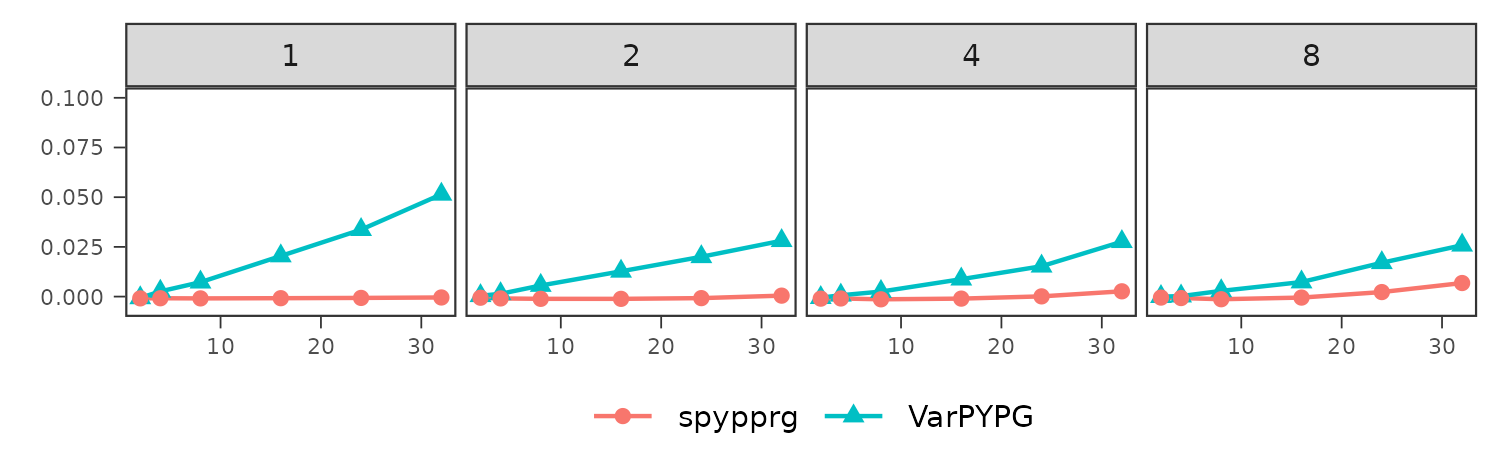
\includegraphics[width=\linewidth]{plots/energy_score}
\end{figure}

To validate the variational model, and investigate the effects of different classes of 
    starting positions, we conduct a simulation study to evaluate various approaches for
    the BNP mixture of projected gammas model.  The datasets are simulated from a finite
    mixture of projected gammas, at varying levels of dimensionality and number of mixture
    components.  For each number of mixture components and dimensionality, 10 sets of
    parameters are generated, and then from for each parameter set, a training dataset and 
    testing dataset, each of \num{1000} replicates, are generated.

As the metric for our evaluation, we use the \emph{energy score} criterion \citep{gneiting2007}
    which is a generalization of the \emph{continuous ranked probability score} to a multivariate
    setting.  This energy score takes the form
    \[
      S_{\text{ES}}(P, \bm{x}) = \text{E}_p\left[g(\bm{X},\bm{x})\right] - 
        \frac{1}{2}\text{E}_p\left[g(\bm{X},\bm{X}^{\prime})\right]
    \]
    where $g$ is a kernel function, $\bm{x}$ is an observed value, and 
    $\bm{X},\bm{X}^{\prime}$ are posterior predictive replicates of $\bm{x}$.
    When energy score is used with an appropriate negative definite kernel 
    metric, it forms a \emph{proper} scoring rule. The specific negative 
    definite kernel we use is described in Prop.~3 of \cite{trubey:pg}, 
    and leverages the fact that all faces of $\mathbb{S}_{\infty}^{d-1}$
    are pairwise adjacent.  By rotating the face of the second point into 
    the same hyperplane as that of the first, the kernel metric becomes the Euclidean 
    distance between the first point, and the rotated second point.
    
Figure~\ref{fig:energyscore} displays the results of our simulation, using the rise in energy score 
    calculated from a posterior predictive sample from the fitted model against the target 
    sample, over a baseline energy score calculated using another random sample from the same 
    generating distribution.  Thus, small values indicate high fidelity of the model in 
    capturing the generating distribution. We investigate this recovery under a variety of 
    conditions increasing the number of dimensions, as well as the number of mixture components 
    in the generating distribution. With this simulation study, we see that
    a pure MCMC approach achieves the best model fidelity, but \emph{VB Pregamed}, using 
    the abridged MCMC sampler to set a starting position for the variational algorithm, 
    achieves a model fidelity that is very nearly indistinguishable from that of the 
    MCMC model.  It also runs significantly faster.
    Note that, as the dimensionality of the problem grows, energy scores become less able to 
    assess model fidelity, as the distance between each observation or replication will approach 
    a constant value \citep{bishop2006}.
    
    % \bruno{\bf We need to indicate that the "MCMC-initialized VB" is better than the
    % MCMC because it is (I guess) faster}

\subsection{Extreme value analysis of SLOSH output\label{sec:slosh}}
As the motivating example for our analysis of the extremal dependence structure, we 
    use the aforementioned SLOSH, which simulates the storm surge resulting 
    from hurricanes over a wide grid.  Our interest is specifically in describing 
    and exploiting the dependence structure of extremes between specific locations.  
    As such, rather than the entire grid, it makes sense to consider data pertaining
    specifically to those locations. 
    % If one is performing contingency planning in preparation for the storm season, 
    % it would be helpful to know the probability of such services being rendered 
    % inoperable simultaneously, precisely when they are needed most.  If one is 
    % seeking sites for a new service provider, it would be helpful understand the 
    % likelihood of a proposed location being rendered inoperable in the same 
    % manner.  For these reasons 
    Thus, we subset the data to grid cells which are in the vicinity of such locations 
    of interest.  We gather these locations from the \emph{point and landmark} file 
    of the US Census Bureau's 2023 \emph{TIGER} database \citep{tiger}.
    We define vicinity as the nearest grid cell within 70 meters of a location---this 
    value stemming from the grid existing on an approximately 110 meter resolution, a 
    70 meter radius ensures no gaps in coverage.
    Additionally, we select grid cells that have experienced at at least some inundation 
    in $q$ proportion of storm simulations.  That is, such that $b_{qs} > 0$, for all 
    $s$ of interest.  This restriction arises as a consequence of fitting the parameters 
    for the marginal generalized Pareto distributions on threshold excesses.
    The quality of MLE estimation of the other marginal GP parameters will suffer if the
    threshold is not well chosen, so to ensure that excesses follow a generalized Pareto,
    we limit analysis to cells that meet this criteria.
    % : if the threshold for excesses $b$ is not set above the minimum observed
    % value in the dataset, MLE estimation of the other marginal GP parameters will suffer.
    Here we suffer another tradeoff, the implications of which are explored in 
    Figure~\ref{fig:thresholdselection}.  Setting a higher quantile threshold allows more 
    sites to be included in the analysis, but in turn reduces the number of storm 
    simulations which exceed the threshold, which in turn reduces the amount of 
    information available by which we can estimate the dependence structure. Using a 
    quantile of \num{0.95}, the resulting number of cells, and number of storm simulations
    exceeding the threshold per slice are summarized in Table~\ref{tab:datasets}.
    % \bruno{\bf This paramgraph is VERY hard to understand. I suppose that you want to
    % say that you are focused on a limited number of locations in the grid of
    % outputs that correspond to key services of infrastructure. }
    % \comment{I have re-written to hopefully make the requirement more clear.}

\begin{figure}[ht]
    \centering
    \caption{Trade-offs in threshold specification:
    (Left) Proportion of sites with threshold $b_{qs} > 0$ versus $(1 - q)$; 
    (Right) Proportion of storms surviving thresholding, $\text{P}(\bm{W}_i \not< \bm{b}_q)$ versus $(1 - q)$.
    \label{fig:thresholdselection}}
    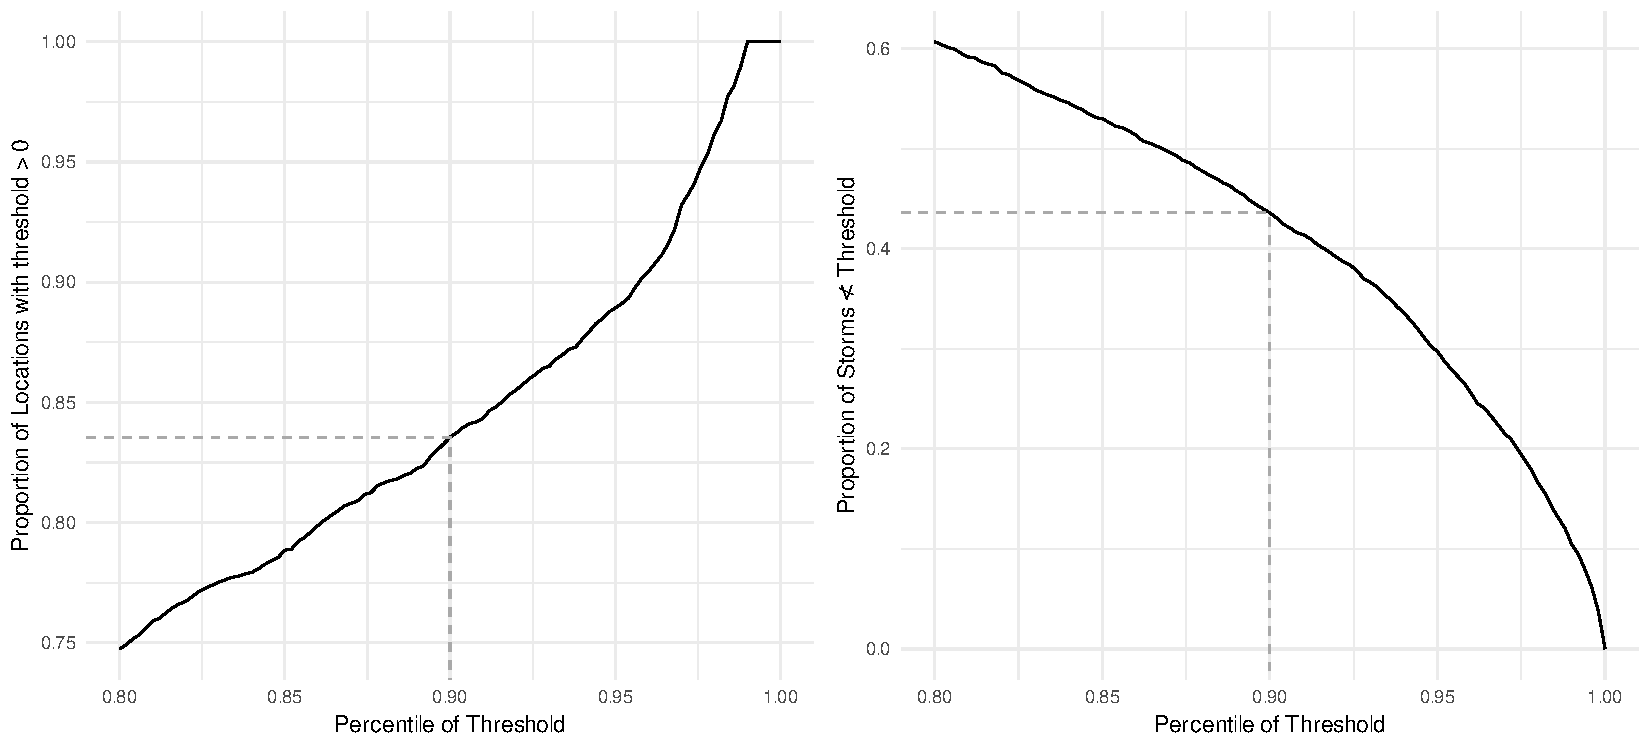
\includegraphics[width=0.7\linewidth]{plots/explore_threshold}
\end{figure}

\begin{table}[htb]
    \centering
    \caption{Slices of SLOSH for analysis.  \emph{Storms} specifies the number of storms that survive 
    thresholding, of the total \num{4000} storms in the sample.  The probability gives that value 
    numerically. \emph{Sites} identifies the number of locations included in the slice. Each 
    subsequent slice is a subset of the preceding slice.\label{tab:datasets}}
    % latex table generated in R 4.4.1 by xtable 1.8-4 package
% Tue Jul 23 14:31:56 2024
\begin{tabular}{lrrrrrrr}
  \hline
Data & Quantile & Cols & Rows & T.05 & T.25 & T.75 & T.95 \\ 
  \hline
Threshold.9 & 0.90 & 4414 & 1744 & 0.39 & 1.64 & 4.58 & 6.19 \\ 
  Limited & 0.95 & 199 & 1040 & 0.38 & 1.84 & 5.13 & 7.00 \\ 
  Transport & 0.95 & 32 & 835 & 0.53 & 1.66 & 5.40 & 6.73 \\ 
  Airports & 0.95 & 27 & 826 & 0.74 & 1.76 & 5.24 & 6.38 \\ 
  Emergency & 0.95 & 6 & 581 & 2.85 & 3.60 & 4.94 & 6.25 \\ 
   \hline
\end{tabular}

\end{table}

% \begin{figure}[htb]
%     \centering
%     \caption{Bounds of storm approach angles.  The eyes of the storms at landing is evenly distributed 
%         in both direction and latitude between the red angles.\label{fig:slosh_bounds}}
%     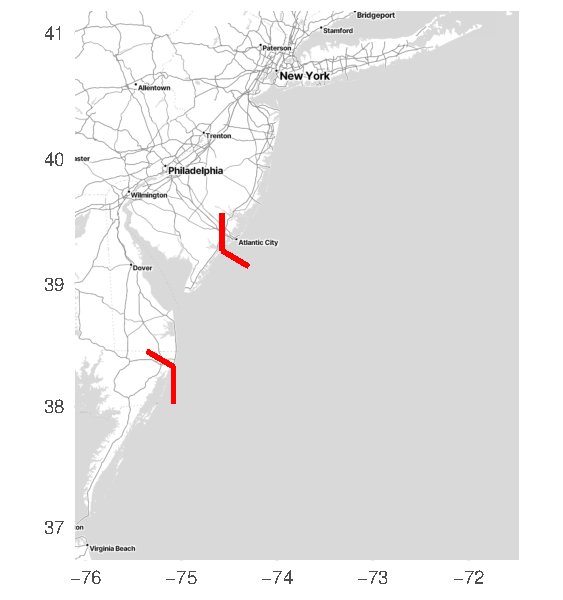
\includegraphics{plots/slosh_bounds}
% \end{figure}

% \st{As previously stated, we require the marginal threshold for excesses to be above 0.  We choose
%     to implement this restriction at the} \bruno{The validity of the proposed PoT model depends on
%     asymptotic results that consider observations above a very large threshold. To define a threshold
%     for each location in the simulation output we take the} 90th percentile \bruno{of the observations
%     per location.}\st{, which defines} \bruno{The resulting thresholded sample corresponds to} the 
%     \emph{Threshold} slice.
%     \makenote{insert data descriptions}.  \bruno{Additional reduction of the sample is produced by
%     considering the bounds of the storm approach angles, one of the SLOSH inputs. }
%     Figure~\ref{fig:slosh_bounds} shows \st{the} \bruno{those} boundaries \bruno{over a portion of 
%     the coastline. We}\st{of  storm approach angles in the SLOSH data---}observe that this 
%     \bruno{is a} rather restricted region, 
%     in comparison to the extent of the data displayed in Figure~\ref{fig:slosh1run},
%     \st{somewhat} \bruno{and} limits the applicability of our methods \st{of analysis in regions outside
%     of} \bruno{to the} Delaware bay and its surrounding area. \bruno{This corresponds to} \st{For this 
%     reason, we restrict our analysis to this region, creating} the \emph{Delaware Bay} slice.  Further 
%     \st{refining analysis to locations} \bruno{refinement of the sample is performed by focusing on 
%     locations}  of particular interest, \st{we} \bruno{identify through the} use the feature class 
%     codes \st{of the locations to isolate} \bruno{that correspond to different} location types
%     \makenote{remove the most common feature classes} of interest.  These form the \emph{Restricted} slice.
%     Finally, we \st{isolate} \bruno{restrict} the data to a few locations of critical interest, 
%     as well as a selection of locations around the bay to inform conditional analysis.  These 
%     form the \emph{Critical} slice. The \st{relative} sizes of \st{these inferential tasks is detailed}
%     \bruno{the different subsamples of the original simulation output, considered in our analysis are
%     reported }in Table~\ref{tab:datasets}.  \st{Having
%     a variety gives us the opportunity to discuss relative strengths of particular types of analysis.}
The validity of the proposed PoT model depends on asymptotic results that consider 
    observations above a very large threshold. To define a threshold
    for each location in the simulation output we take the 90th percentile 
    of the observations per location.  The resulting thresholded sample corresponds to
    the \emph{Threshold} slice.  Additional reduction of the sample is produced by
    considering the bounds of the storm approach angles, one of the SLOSH inputs. 
    Figure~\ref{fig:slosh_bounds} shows those boundaries over a portion of 
    the coastline. We observe that this is a rather restricted region, 
    in comparison to the extent of the data displayed in Figure~\ref{fig:slosh1run},
    and limits the applicability of our methods to the Delaware bay and its 
    surrounding area. This corresponds to the \emph{Delaware Bay} slice.  Further 
    refinement of the sample is performed by focusing on locations of particular 
    interest, identified through the use the feature class codes that correspond 
    to different location types of interest.  These form the \emph{Restricted} slice.
    Finally, we restrict the data to a few locations of critical interest, 
    as well as a selection of locations around the bay to inform conditional analysis.  
    These form the \emph{Critical} slice. The \st{relative} sizes of the different 
    subsamples of the original simulation output, considered in our analysis are
    reported in Table~\ref{tab:datasets}.

\begin{figure}[htb]
    \centering 
    \caption{Histograms of characteristics for simulations that survived thresholding in \emph{Threshold}.
        Sea level rise in mm, approach angle in degrees, approach speed in Kph, minimum pressure in mBar,
        latitude in decimal degrees. \makenote{Make this a pairs plot?}
        \label{fig:thetahistogram}}
    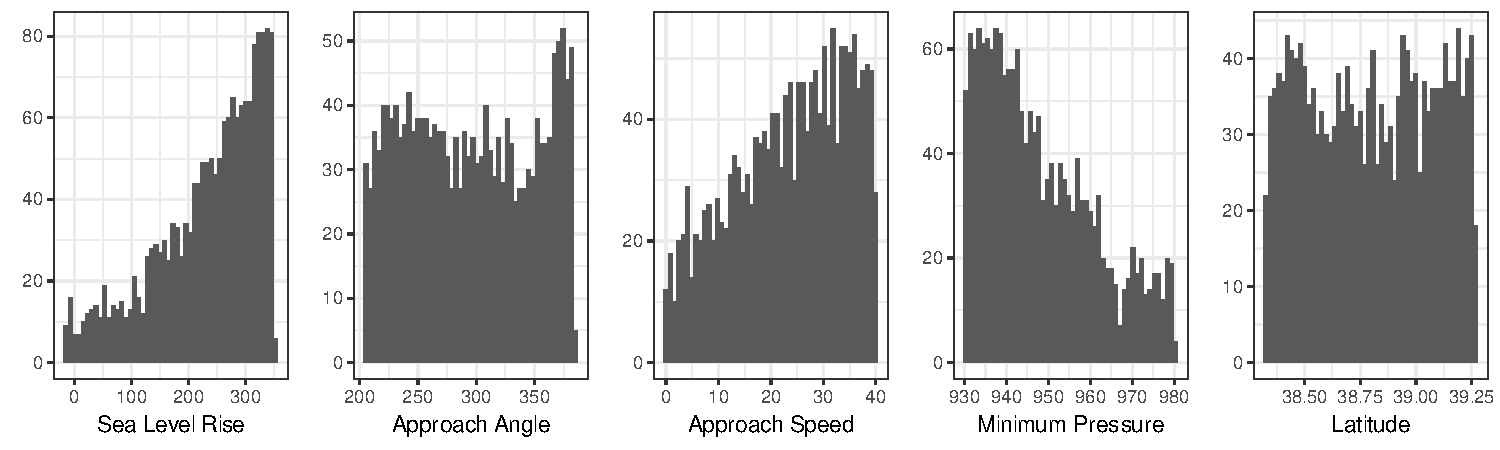
\includegraphics[width=0.9\linewidth]{plots/threshold_histogram}
\end{figure}

Figure~\ref{fig:thetahistogram} shows the marginal histograms of SLOSH input 
    parameters, for storms which exhibited extreme behavior in the \emph{Threshold} 
    slice.  Storm parameters in the original simulation were sampled via Latin 
    hypercube, so would appear marginally uniform.  The difference between marginal 
    uniform, and the observed densities provides some indication of what 
    characteristics are necessary for a storm to exceed the threshold.
    Imprimis, for sea level rise it is readily apparent that a higher sea level will
    make it easier for a storm to inundate larger swaths of land, or inundate locations to a
    greater degree.  So we expect and, in fact, see a higher proportion of storms exceeding
    the threshold, for a higher sea level rise.  Similarly, a lower minimum pressure in the storm's
    eye corresponds to a more powerful storm.  This bears out, as a lower minimum pressure has
    a higher probability of exceeding the threshold.  The relationship to approach speed is 
    interesting in that it is nearly linear.  Perhaps, the mechanism there lies in that a higher
    approach speed indicates more power behind the storm.  The spike in approach angle past 360
    degrees is interesting as well. 360 degrees indicates due North, thus approach angles 
    beyond 360 degrees indicate the storm is heading slightly northeast. As these approaches are
    on the eastern seaboard, this means a shallower approach angle relative to the
    land---perhaps offering a given storm more time to inundate larger swaths of land.

% EOF 